Pour optimiser tous nos paramètres, autant pour les objets de compte que pour les modèles de classification, on calcule le score défini à la section précédente pour plusieurs combinaisons de paramètres possibles. Voici les paramètres choisis pour ces tests:

\begin{description}
\item \textbf{SVM}(Support Vector Machine): valeur de C, type de noyau (kernel)
\item \textbf{KPPV} (K plus proche voisins): nombre de voisins k, type de poids
\item \textbf{Régression Logistique}: type de pénalité appliquée
\item \textbf{MLP} (Multi Layer Perceptron): nombre de neurones pour chaque couche cachée.
\end{description}
Voici les listes des valeurs choisies pour notre recherche en grille:

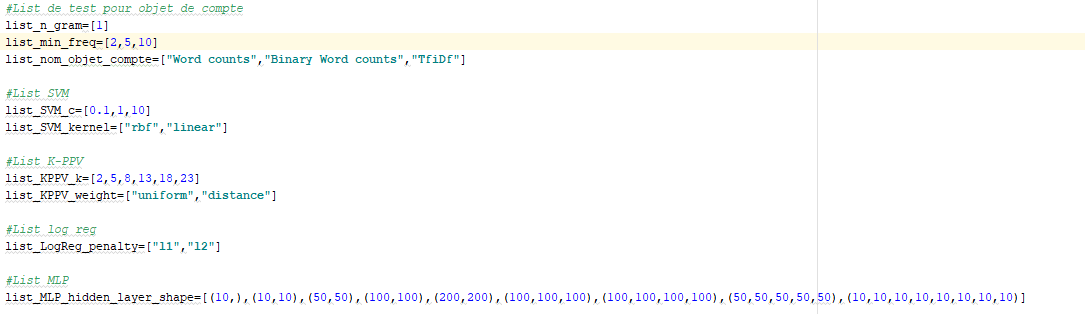
\includegraphics[width=\linewidth,height=8cm]{images/list_param}

Cela fait donc $(3*3*3) *(3*2 + 6*2 + 2 + 9)=783$ combinaisons de paramètres à tester. La combinaison ayant le meilleur score est sauvegardée dans le fichier \emph{Dictionnaire\_parametre\_meilleur\_model} sous la forme d'un dictionnaire contenant ses paramètres. 
Le dictionnaire prend la forme suivante: \{nom du classificateur, score, dictionnaire de paramètres du classificateur, nom du modèle de compte, dictionnaire de paramètres du modèle de compte\}.